% label prefix for this part: pm
\part{Projektmanagement}

\chapter{Vorgehensmodell}

Das gesamte Projekt wird im Stil von RUP geführt und dementsprechend in die vier Phasen Inception, Elaboration, Construction und Transition aufgeteilt. In der Construction-Phase wird nach agiler Vorgehensweise gearbeitet, so dass der Auftraggeber die Schwerpunkte setzen und priorisieren kann.

\xxx[Grafik?]

\chapter{Rollen und Verantwortlichkeiten}

An diesem Projekt arbeiten die beiden unten aufgeführten Informatik-Studenten. Aufgrund der entsprechenden Stärken und beruflichen Orientierungen übernimmt Philipp Christen die Verantwortung über das Frontend, Ueli Bosshard übernimmt die Verantwortung über das Backend und die Kommunikation mit apt.

\xxx[Fotos]

\begin{tabular}{ | l | l | }
    (Foto) & (Foto) \\
    Ueli Bosshard & Philipp Christen \\
    Stärken: Systemtechnik, OS, Netzwerk, DB
    &
    Stärken: Frontend, UX\\
\end{tabular}

\chapter{Risiken}\label{sec:risiken}

Um die potentiellen Risiken während des Projekts zu sammeln, wurde eine  Risiko-Checkliste verwendet. Für jedes Risiko wurde ein zusätzlicher Aufwand in Stunden geschätzt, welcher anfallen würde wenn das Risiko eintritt. Multipliziert mit der geschätzten Eintrittswahrscheinlichkeit ergab dies einen gewichteten Mehraufwand. Dieser wurde in 5 Kategorien (sehr gering bis sehr schwer) eingestuft.

Ziel war es, alle Risiken bis Ende Elaborations-Phase entweder komplett auszuschliessen oder soweit zu Entschärfen, dass beim Eintreten Sicherheitsmassnahmen greifen und keine grosse Verzögerung oder anderen Schaden verursachen.

Es wurden nur für das Projekt relevante Risiken analysiert. Risiken wie "Krankheit" wurden absichtlich nicht notiert, da es hier keine sinnvollen Präventionsmassnahmen gibt.

\xxx[Check Tempus!]

\begin{landscape}
	\begin{table}[H]
		\centering
		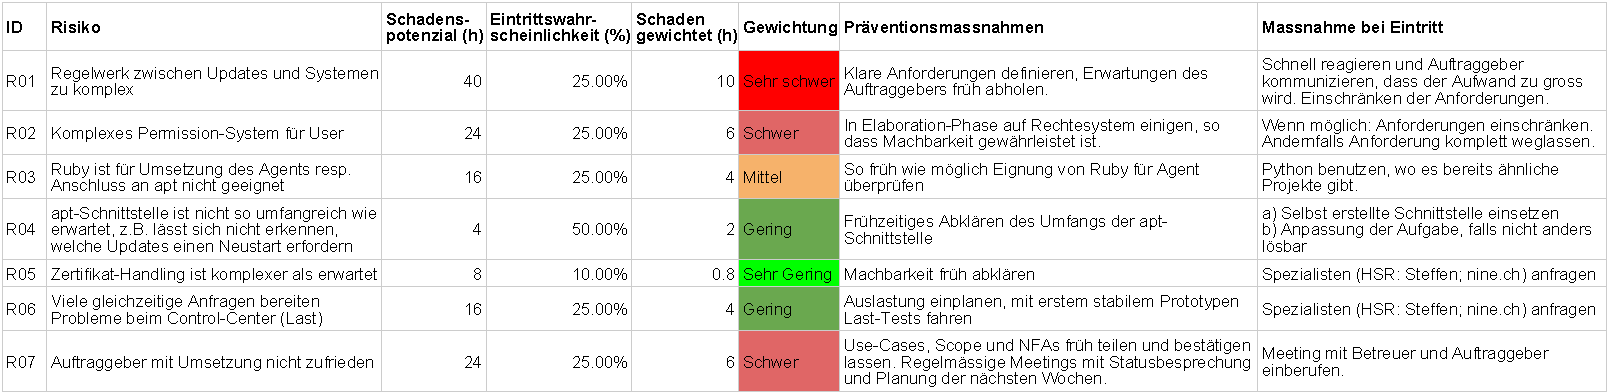
\includegraphics[width=0.8\textwidth,keepaspectratio]{Risikoanalyse.pdf}
		\caption{Alle berücksichtigten Risiken}
		\label{tab:risikoanalyse}
	\end{table}
\end{landscape}

\section{Kritische Risiken}

Die besonders kritischen Risiken werden hier kurz erläutert und genauer beschrieben.

\newcommand{\projectrisk}[4]{
	\begin{tabularx}{\linewidth}{lX}
		\toprule
		\textbf{Risiko} & #1\\
		\midrule
		\textbf{Titel} & #2\\
		\textbf{Beschreibung} & #3\\
		\textbf{Prävention/Massnahme} & #4\\
		\bottomrule
	\end{tabularx}
}


\projectrisk{R01}{Regelwerk zwischen Updates und Systemen zu komplex}
{Es war von Beginn an nicht klar, wie genau das Regelwerk genau aussehen soll, welches die Kombinationen von Systemen und Updates einschränken soll. Im schlimmsten Fall können es beliebig tiefe Abhängigkeiten sein, welche über mehrere Gruppen hinweg geprüft werden müssen.}
{In der Elaborations-Phase sollte so gut wie möglich geklärt werden, in welcher Form das Regelwerk entstehen soll. Sobald sich herausstellt, dass die gewählte Tiefe der Umsetzung zu viel Aufwand verursacht, wird mit dem Auftraggeber entschieden, ob die Anforderung gegebenfalls eingegrenzt werden kann.}


\projectrisk{R02}{Komplexes Permission-System für User}
{Wie beim Regelwerk zwischen Updates und Systemen können die Berechtigungen der Benutzer beliebig fein konzeptioniert werden. Dadurch müssen nicht nur die Berechtigungen selbst geprüft werden, sondern auch Abhängigkeiten unter den Berechtigungen - es ist sinnlos, wenn man einem Benutzer das Updaten einer spezifischen Gruppe verbietet, aber das Erstellen und Bearbeiten einer Gruppe erlaubt ist.}
{Wiederum soll in der Elaboration-Phase mit dem Auftraggeber das Rechtesystem vereinbart werden, so dass die Machbarkeit gewährleistet ist. Falls dies nicht gelingt oder sich als schwerer als geplant entpuppt, sollen wenn möglich die Anforderungen eingeschränkt werden. Falls es keine brauchbare Lösung gibt, muss auf das Rechtesystem verzichtet werden.}


\projectrisk{R07}{Auftraggeber mit Umsetzung nicht zufrieden}
{Der Auftraggeber kann trotz korrekter Umsetzung mit dem Endresultat nicht zufrieden sein, etwa indem implizite und nicht dokumentierte Annahmen von Kundenseite her nicht oder nur teils erfüllt wurden.}
{Es soll früh abgegrenzt werden, was genau zum Projektumfang gehört, welche Use-Cases und NFAs gelten und welche Features implementiert werden. Dies soll vom Auftraggeber bestätigt werden. Regelmässige Meetings mit Statusbesprechung und Planung der nächsten Wochen sollen unterschiedliche Vorstellungen verhindern und alle Parteien am Entstehungsprozess beteiligen lassen. Falls trotzdem Unzufriedenheit auftreten sollte, muss dies zusammen mit dem Betreuer genauer angeschaut werden.}


\chapter{Infrastruktur}

Da es sich um ein Open-Source-Projekt handelt, wurde der Quellcode veröffentlicht. Bereits während der Entwicklung war er jederzeit auf Github\footnote{\purl{https://github.com/upd89/}} einsehbar.

\xxx[similar chart would be sweet]

\begin{figure}[H]
	\centering
	\includegraphics[width=\linewidth]{fig/entwicklungsumgebung}
	\caption{Entwicklungsumgebung}
	\label{fig:pm:entwicklungsumgebung}
\end{figure}

\section{Projektmanagement}



\chapter{Qualitätsmanagement}

\xxx

\subimport{sprints/}{sprints.tex}
